This chapter describes the seismic source typologies supported by the OQ-engine: \textit{Point} and
\textit{Area} sources for modeling distributed seismicity, \textit{Simple Fault}, \textit{Complex Fault}, and
\textit{Characteristic Fault} for modeling fault-based seismcity.


\section{Basic concepts}
%------ The different source typologies ------%
%------ Point and Area ----------%
The OQ-engine provides several seismic source typologies to accomodate different modeling approaches. For modeling distributed seismicity, that is seismic activity occurring over a geographilcal region and not tight to
specific well characterized fault structures, the OQ-engine provides the \textit{Point} and \textit{Area} sources. The former defines seismic activity \textit{nucleating in a single geographical location}, while the second seismicity occurring \textit{uniformly over a geographical region}. Both sources define a seismogenic layer which constrains rupture location and extension along depth. A collection of Point sources can be used to model seismicity with spatially variable parameters (as obtained from a smoothed seismicity approach for instance), while Area sources can be used to model seismicity in geographic zones usually defined by expert judgments taking into account seismological, geological and geodetic information. Both source typologies
allows modeling earthquake ruptures as extended surfaces (that is as plane rectangles in a 3D space) with potentially multiple orientations and inclinations (that is multiple strike and dip angles) and also placed
at different depth levels. Earthquake ruptures can extend without barriers along strike but cannot cross the seismogenic layer.\\
%------- Faults ---------%
For modeling fault-based seismicity, that is seismic activity occurring on a well identified and characterized
fault zone, the OQ-engine provides two main options, the \textit{Simple Fault} and the \textit{Complex Fault}
sources. Both source typologies allows distributing seismicity \textit{uniformly over a fault surface}, with the
only constrain that an earthquake rupture cannot extend outside of the defined fault surface. In both sources an earthquake of a given magnitude is defined as a portion of the fault surface. To simulate all possible rupture locations, an earthquake rupture is \textit{floated}, that is moved, over the entire fault surface. The two source typologies differs instead in terms of the geometrical complexity they can accomodate when modeling a fault surface. In particular, a Simple Fault source can model a fault surface as a plain rectangle in the simplest case, or as a set of connected parallelograms in the most complex case. A Complex Fault source can instead model an arbitrarily complex quadrilateral surface, which can therefore accomodate changes in dip angle along depth or along strike or changes in fault width. The Complex Fault source is therefore particularly suitable for modeling large subdution interface faults, while Simple Fault sources can be used for modeling crustal faults. The \textit{Characteristic Fault} source can model both simple and complex geometries, but instead of simulating floating ruptures, each earthquake breaks the entire fault surface indipendently of the associated magnitude. The Characteristic Source typology can be used to model individual faults or fault segments that tend to produce essentialy same size earthquakes (CITE SCHWARTZ COPPERSMITH 1984).\\
%-------- Common parameters -------%
%-------- Magnitude-Frequency Distribution-------%
Indipendently of the typology, all sources require the definition of the following main parameters:
\begin{itemize}
\item magnitude-frequency distribution
\item tectonic region type
\item magnitude-area scaling relationship (for all but the Characteristic Fault source)
\item rupture-aspect ratio (for all but the Characteristic Fault source)
\item upper seismogenic depth
\item lower seismogenic depth
\end{itemize}
The magnitude-frequency distribution defines the total moment rate released by a source. It is therefore a
key parameter which determines the influence of a source in a PSHA. The OQ-engine supports the definition
of the traditional \textit{double-truncated Gutenberg-Richter} magnitude-frequency distribution which is
widely used in any PSHA. Required parameters are the cumulative \textit{a-value} (defined as the intercept
of the \textit{cumulative} distribution at $M=0$ in a $log10$ scale), the $b-value$, the minimum and
the maximum magnitudes. However, to accomodate also other possibile parametric (and non-parametric)
forms, the OQ-engine provides a generic discrete \textit{Incremental} magnitude-frequency distribution
defined through a list of annual occurrence rates, associated to an equally spaced set of magnitude values.\\
In a PSHA, the magnitude-frequency distribution is subject to a discretization process which defines a set
of equally spaced magnitude bins and the associated annual occurrence rates (for an \textit{Incremental}
magnitude-frequency distribution such a discretization is part of its definition). For each source, the annual
occurrence rate associated to a magnitude bin is \textit{uniformly} distributed over all the ruptures associated
to the same magnitude bin value. In other words, while the particular geometry of a source determines
location and number of ruptures of a given magnitude, the occurrence rate (and thus the occurrence
probability) is uniform over ruptures with the same magnitude.\\
%----------Tectonic Region Type---------%
The second typology-indipendent parameter associated to a seismic source is the tectonic region type.
This is a source attribute which is used as a key to associate a seismic source to a ground motion model.
Given a source model describing seismicity occurring in a region where different tectonic settings overlap or
are close to each other, the associated ground motion model may prescribe different equations for the different
tectonic settings. The mapping between a ground motion model equation and a seismic source is therefore
achieved through the tectonic region type attribute.\\
%-----------Magnitude-Area Scaling and Rupture Aspect Ratio----------%
All sources model earthquake ruptures as extended surfaces. With the only exception of the Characteristic Fault source, the area of an earthquake rupture surface is magnitude dependent. To constrain the rupture surface area, the Point, Area, Simple and Complex Fault sources require the definition of a \textit{magnitude-area} scaling relationship. Together with a \textit{rupture aspect ratio} (defined as ratio between length and width), the rupture extension and shape (assumed rectangular) is completely defined. Indeed, indicating with $A$ the rupture area and with $ar$ the rupture aspect ratio, rupture length ($L$) and and width ($W$) can be computed as:
\begin{equation}
\begin{split} \label{eq:rup_l_w}
&L = \sqrt{A * ar}  \\
&W = \sqrt{A / ar}
\end{split}
\end{equation}
In all sources, the rupture aspect ratio is used to constrain the initial rupture shape. However, if this conflicts with other source-dependent geometrical constrains, the rupture is reshaped so as to conserve the area as given by the scaling relationship.\\
%-----------Upper and Lower Seismogenic Depths-------------%
The upper and lower seismogenic depths define the seismogenic layer, that is the depth range over which earthquake ruptures can occur. The definition of a seismogenic layer is required to avoid an uncontrolled extension of the earthquake ruptures along depth which can lead, especially for large magnitude events, to unrealistic scenarios. The definition of a seismogenic layer thickness effectively induces a magnitude-dependent rupture aspect ratio. Indeed, as the rupture size increases with increasing magnitude values, the rupture width reaches the maximum allowed width, and the rupture aspect ratio starts deviating, that is increasing, from the original value.

\section{The Point and Area sources}
The parameters specific to the definition of Point and Area sources, and their associated function, are listed in Table \ref{table:point_area_tab}.
\begin{table}
\caption{Table summarizing parameters, and their functions, required for the definition of Area and Point
sources in the OQ-engine}
\centering
\begin{tabular}{p{60mm} p{60mm}}
\specialrule{.2em}{.1em}{.4em} 
Parameter & Purpose \\ [0.5ex] % inserts table
\specialrule{.2em}{.1em}{.4em}
Magnitude frequency distribution & Defines total moment rate\\ 
\specialrule{.05em}{.1em}{.4em}
Magnitude area scaling relationship & Define sizes and shapes of rupture planes \\
Rupture aspect ratio (length / width) & \\
\specialrule{.05em}{.1em}{.4em}
Nodal plane distribution \newline (each nodal plane being defined \newline by strike, dip, rake) & Defines orientations and faulting styles of ruptures \\
\specialrule{.05em}{.1em}{.4em}
Hypocentral depth distribution &  Defines centroids of rupture planes \\
\specialrule{.05em}{.1em}{.4em}
Upper seismogenic depth & Constrains rupture planes inside seismogenic layer \\
Lower seismogenic depth & \\
\hline %inserts single line
\end{tabular}
\label{table:point_area_tab}
\end{table}
Sources are parameterized so that earthquake ruptures are modeled as planar rectangles in a 3D space. In a point-source representation (Figure \ref{fig:PointSource}) ruptures are generated underneath a single geographical location, and can be potentially distributed over multiple orientations, faulting styles, and depth levels.
\begin{figure}
\centering
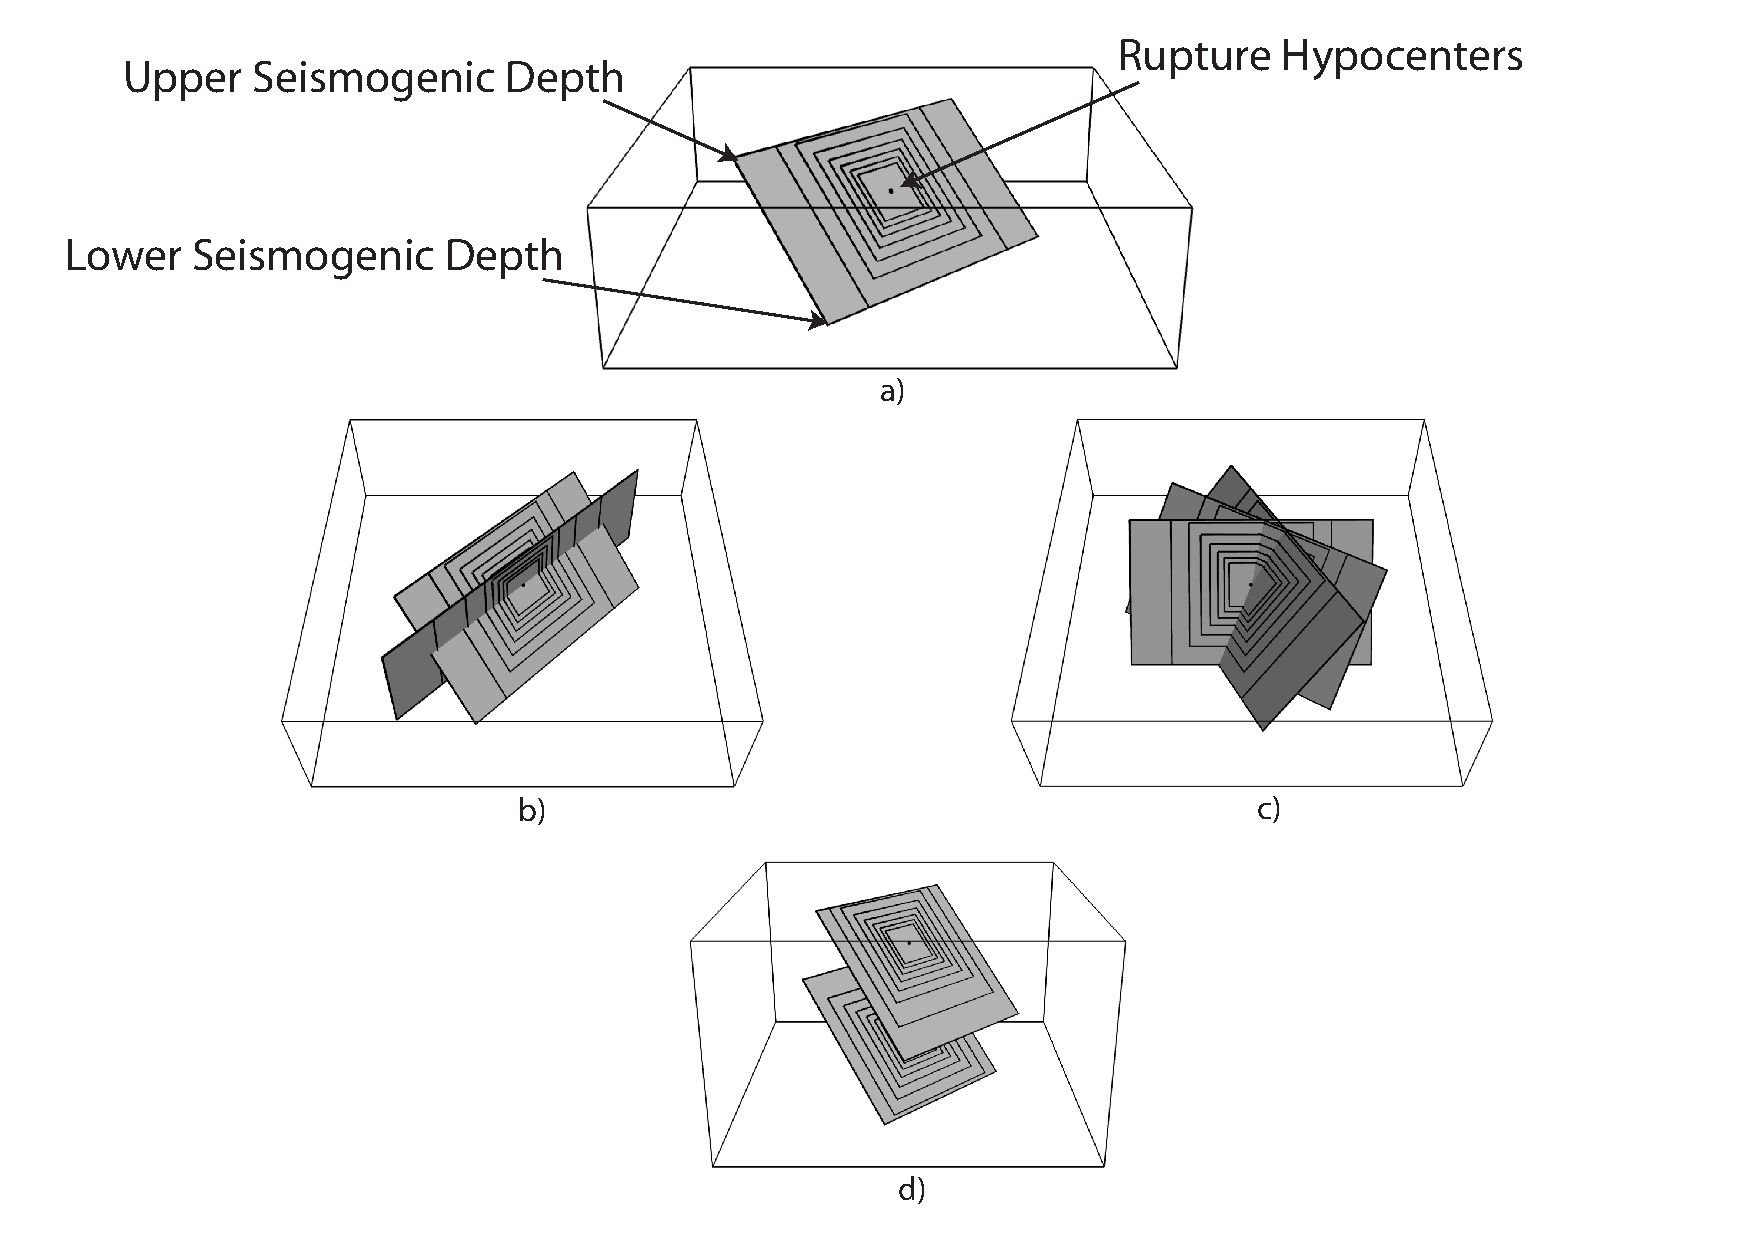
\includegraphics[width=14cm]{./Pictures/PointSource.pdf}
\caption{Graphical representation of the earthquake ruptures as generated by a Point Source. a) Given a geographical location on the earth surface, ruptures are generated underneath according to a scaling relationship and aspect ratio value and forced to not exceed the upper and lower seismogenic depths. Ruptures can be distributed over multiple dips b), strikes c) and hypocentral depths d).}
\label{fig:PointSource}
\end{figure}
Rupture centroids are co-located with the point-source location and are positioned at depths specified by the hypocentral depth distribution. Rupture shapes follow the given aspect ratio. However, if for a given aspect ratio and hypocentral depth the rupture plane crosses either boundary (upper or lower) of the seismogenic layer, the plane is shifted along the dip direction so as to fit within the upper and lower seismogenic depths. As a consequence, the hypocentral location no longer corresponds with the plane centroid. If this adjustment is insufficient to avoid crossing either boundary of the seismogenic layer, the plane is reshaped; the width becomes the maximum allowed by the seismogenic layer thickness, and the length is increased so as to conserve rupture area (at the expense of the aspect ratio).\\
In an area source (Figure \ref{fig:AreaSource}), earthquake ruptures are distributed over a regular grid (equally-spaced in distance) covering a geographical region as defined by a seismic zone. 
\begin{figure}
\centering
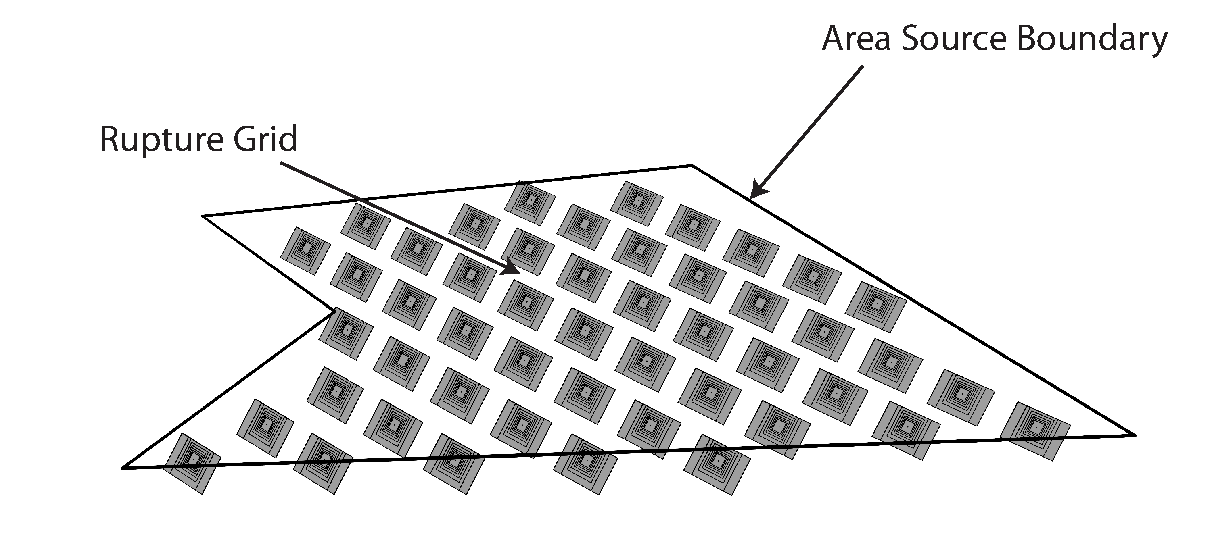
\includegraphics[width=14cm]{./Pictures/AreaSource.pdf}
\caption{Earthquake ruptures generated by an area source in the OQ-engine. Ruptures are distributed uniformly over a regular grid within the area. In this plot, for better visualization, ruptures are modeled only according to a single nodal plane and hypocentral depth, but actual calculations may involve multiple orientations and hypocentral depths. Ruptures originating from different grid nodes may also overlap and cross each other.}
\label{fig:AreaSource}
\end{figure}
Generation of ruptures follows the same algorithm as for point sources. For both sources, the rate associated to each rupture plane is the original rate associated to the corresponding magnitude bin, scaled by the location weight (1 for a point source and 1 / N for an area source, where N is the total number of grid points in the area), the nodal plane (that is orientation and faulting style) weight, and the hypocentral depth weight.\\
For an area source, the boundary is assumed ‘leaky’, that is earthquake ruptures can extend out of it. Because of rupture area conservation, earthquake surfaces associated to large magnitudes can extend well beyond the source boundaries. If the rupture orientation is considered random then this behavior can potentially lead to unrealistic scenarios, that is earthquake ruptures that are not consistent with the area geometry and the tectonic feature it is meant to represent. The design of an area source requires therefore a careful estimation not only of the associated activity rates but also of the predominant faulting orientations.\\
\section{The Simple Fault source}
Parameters required for the definition of a Simple Fault source are given in Table \ref{table:simple_fault_tab}.
\begin{table}
\caption{Table summarizing parameters, and their functions, required for the definition of a Simple Fault source in the OQ-engine}
\centering
\begin{tabular}{p{60mm} p{60mm}}
\specialrule{.2em}{.1em}{.4em} 
Parameter & Purpose \\ [0.5ex] % inserts table
\specialrule{.2em}{.1em}{.4em}
Magnitude frequency distribution & Defines total moment rate\\ 
\specialrule{.05em}{.1em}{.4em}
Magnitude area scaling relationship & Define sizes and shapes of rupture planes \\
Rupture aspect ratio (length / width) & \\
\specialrule{.05em}{.1em}{.4em}
Fault trace & Define fault surface \\
Upper seismogenic depth & \\
Lower seismogenic depth & \\
Dip angle & \\
\specialrule{.05em}{.1em}{.4em}
Rake angle & Defines faulting style \\
\hline %inserts single line
\end{tabular}
\label{table:simple_fault_tab}
\end{table}
The fault surface is constructed by translating the fault trace from the upper to the lower seismogenic depth along a direction perpendicular to the fault trace (measured as the difference between the azimuths of the first and last coordinates of the trace) and with an inclination equal to the dip angle. The surface so defined is
effectively modeled as a regular (i.e. equally spaced in distance) mesh [Figure
\ref{fig:SimpleFaultSource} a)].
\begin{figure}
\centering
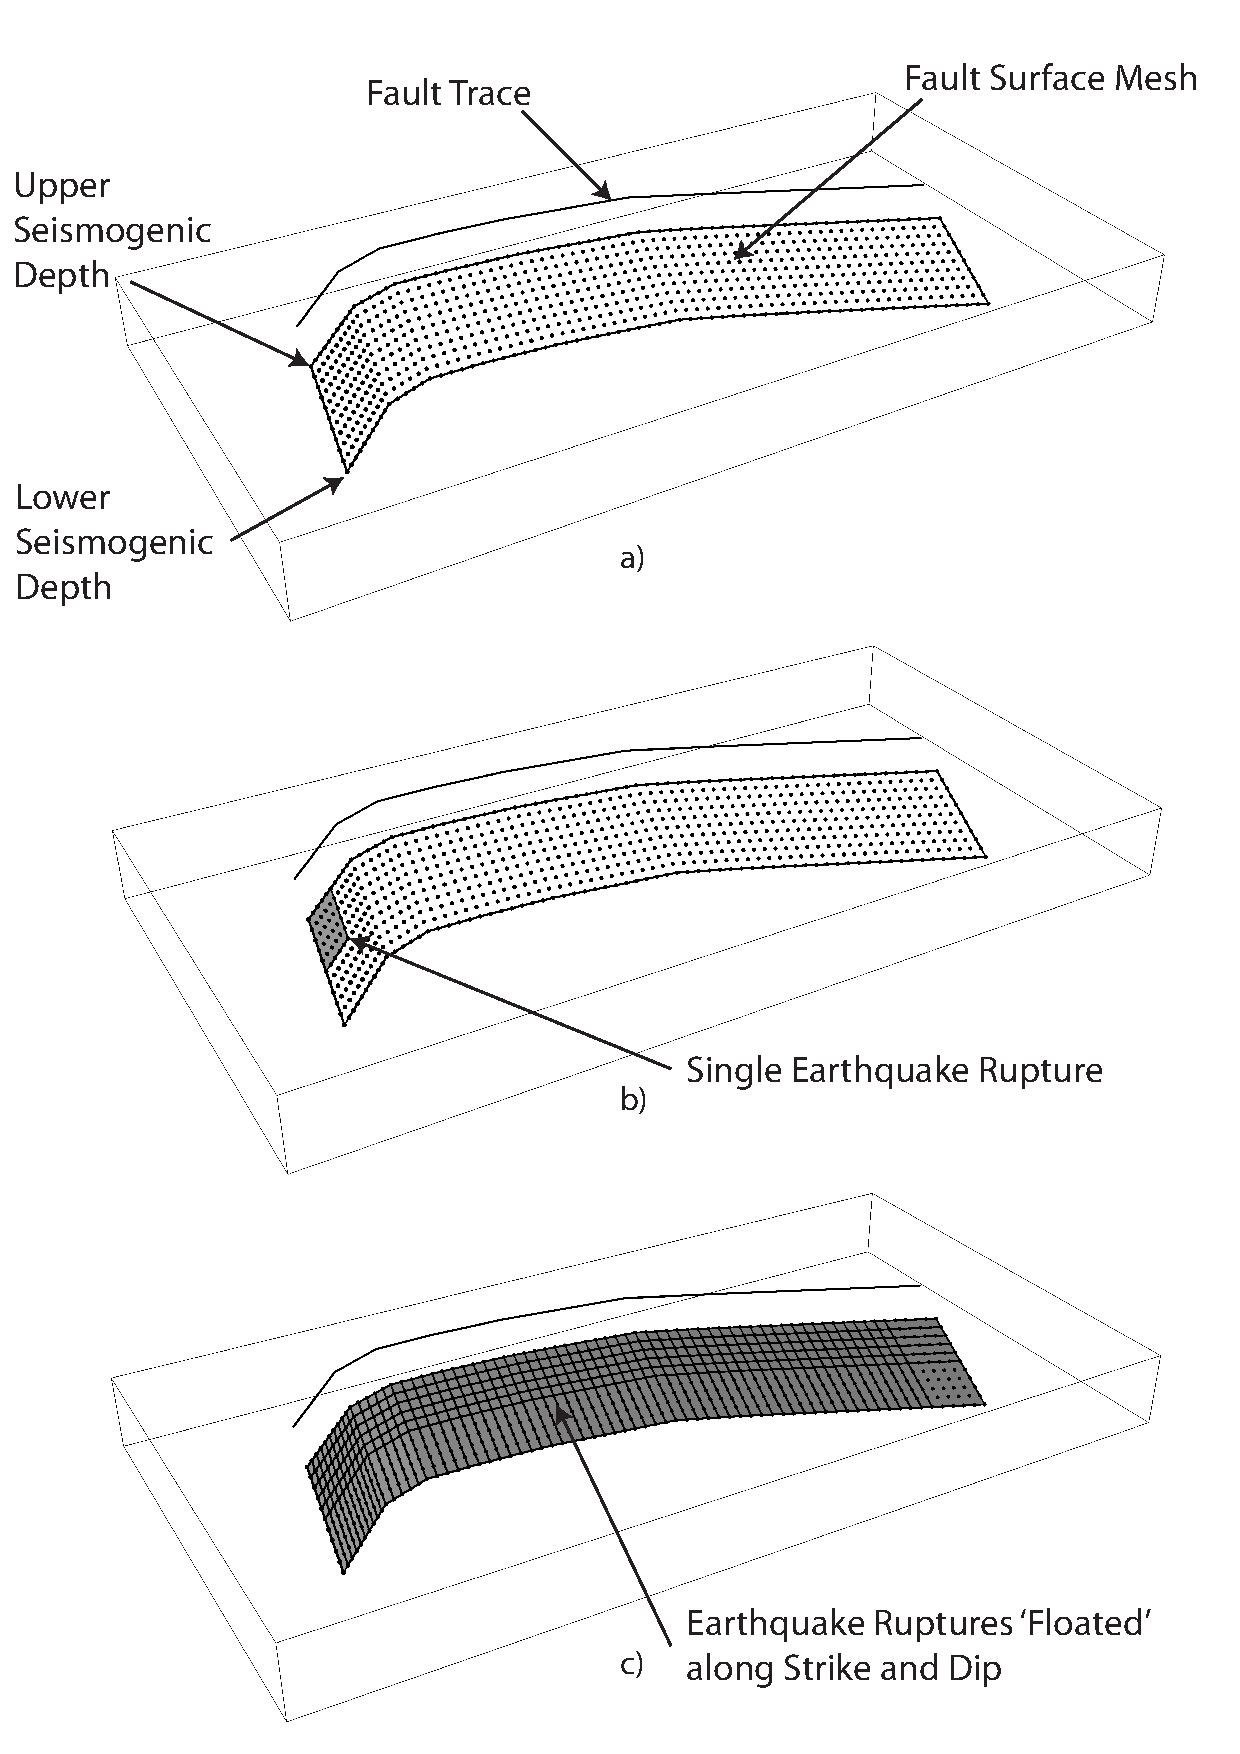
\includegraphics[width=14cm]{./Pictures/SimpleFaultSource.pdf}
\caption{Simple Fault source in the OQ-engine. a) Mesh representation of the fault surface, b) Single earthquake rupture on the fault surface, c) Earthquakes floated over the fault surface}
\label{fig:SimpleFaultSource}
\end{figure}
For each magnitude bin defined in the magnitude-frequency distribution, an earthquake rupture is modeled as a portion of the fault surface, accordingly with the magnitude scaling relationship and the rupture aspect
ratio [Figure \ref{fig:SimpleFaultSource} b)]. To simulate all possible rupture locations, each earthquake rupture is \textit{floated}, that is moved, along both the strike and dip directions [Figure
\ref{fig:SimpleFaultSource} c)]. The floating step is assumed equal to the mesh discretization step.
The occurrence rate associated to a given magnitude bin is distributed uniformly over all the ruptures associated with the same magnitude value.
\subsection{The rupture floating algorithm for a Simple Fault source}
We describe here in more detail the algorithm adoped for modeling floating ruptures in a Simple Fault source. We indicate with $\Delta$ the mesh spacing, and with $n_{strike}^{fault}$ and $n_{dip}^{fault}$ the number of nodes along the strike and dip directions in the mesh representing the entire fault surface. By indicating with $L(M)$ and $W(M)$ the length and width of a rupture of magnitude $M$ (obtained from equation \ref{eq:rup_l_w}), the equivalent number of nodes (along strike and dip) representing a rupture on the mesh can be computed as:
\begin{equation} \label{eq:rup_nodes}
\begin{split}
& n_{strike}^{rup}(M) =  L(M) / \Delta + 1 \\
& n_{dip}^{rup}(M)     = W(M) / \Delta + 1 
\end{split}
\end{equation}
By further assuming that a rupture is floated along strike and dip with a step equal to the mesh spacing ($\Delta$), we can compute the total number of ruptures along strike and dip as:
\begin{equation}
\begin{split}
& N_{rup}^{strike}(M) = n_{strike}^{fault} - (n_{strike}^{rup}(M) - 1) \\
& N_{rup}^{dip}(M)     = n_{dip}^{fault} - (n_{dip}^{rup}(M) - 1)
\end{split}
\end{equation}
That is a rupture can propagate until its boundary reaches the fault boundary, but not beyond. Therefore the total number of possible rupture locations along a certain dimension is equal to the total number of nodes minus the number of nodes required by the rupture reduced by 1, which represents the number of positions that a rupture
cannot occupy because it would otherwise extend, at least of one mesh spacing, outside of the fault boundary.
Indicating with $\nu(M)$ the annual occurrence rate as given by the magnitude-frequency distribution, the annual occurrence rate associated to each rupture of magnitude $M$ is given by:
\begin{align}
\nu_{rup}(M) = \frac{\nu(M)}{N_{rup}^{strike}(M) * N_{rup}^{dip}(M)}
\end{align}
The occurrence rate scaling factor is therefore magnitude dependent (in contrast with the Area Source where the scaling is constant for all magnitudes).

\section{The Complex Fault source}
Parameters required for the definition of a Complex Fault source are given in table \ref{table:complex_fault_tab}.
\begin{table}
\caption{Table summarizing parameters, and their functions, required for the definition of a Complex Fault
source in the OQ-engine}
\centering
\begin{tabular}{p{60mm} p{60mm}}
\specialrule{.2em}{.1em}{.4em} 
Parameter & Purpose \\ [0.5ex] % inserts table
\specialrule{.2em}{.1em}{.4em}
Magnitude frequency distribution & Defines total moment rate\\ 
\specialrule{.05em}{.1em}{.4em}
Magnitude area scaling relationship & Define sizes and shapes of rupture planes \\
Rupture aspect ratio (length / width) & \\
\specialrule{.05em}{.1em}{.4em}
Top edge & Define fault surface \\
Intermediate edges (optional) & \\
Bottom edge & \\
\specialrule{.05em}{.1em}{.4em}
Rake angle & Defines faulting style \\
\hline %inserts single line
\end{tabular}
\label{table:complex_fault_tab}
\end{table}
To accomodate the definition of irregular geometries, the Complex Fault source requires the
specification of the coordinates of, at leats, the top and bottom edges of the fault surface, and
optionally, of one or more intermediate edges [Figure \ref{fig:ComplexFaultSource} a)]. Edges
can have different and variable directions and a single edge can develop over different depth levels.
This gives a very large flexibility in the definition of the fault surface, allowing for changes in width
and inclination both along strike and along dip.
\begin{figure}[!ht]
\centering
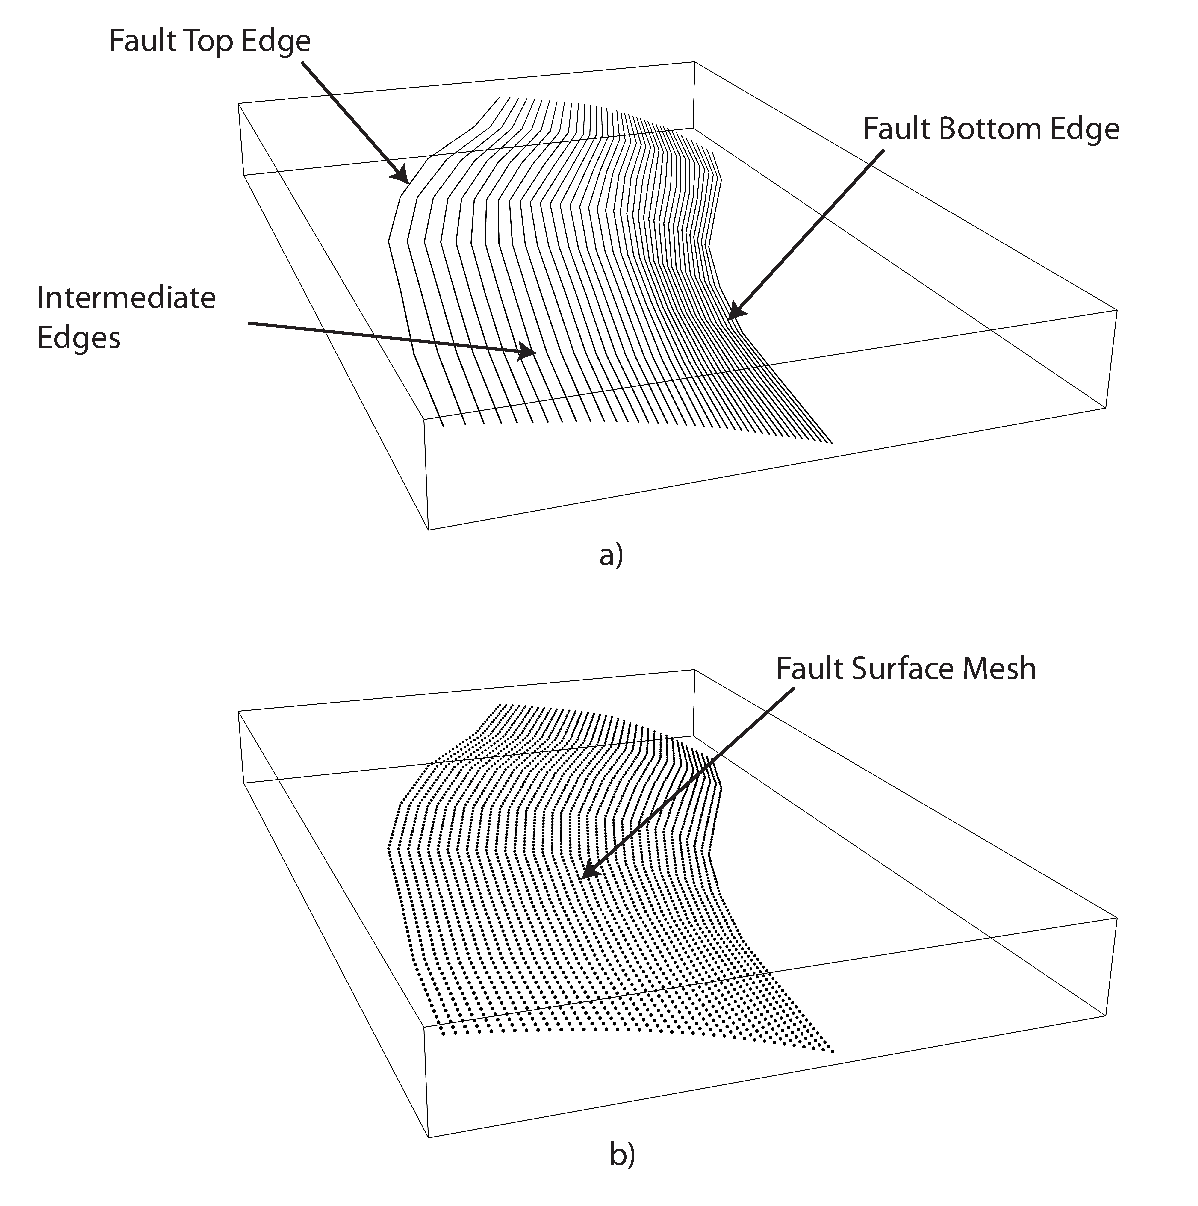
\includegraphics[width=14cm]{./Pictures/ComplexFault.pdf}
\caption{Complex Fault source}
\label{fig:ComplexFaultSource}
\end{figure}

\subsection{Mesh construction in a Complex Fault source}
The fault edges are used to construct a mesh representing the fault surface 
[Figure \ref{fig:ComplexFaultSource} b)]. The mesh is, in general, not uniform; that is,
the mesh spacing may be spatially variable to accomodate the irregular geometry of the surface.
The construction of the mesh rely on the following algorithm. By indicating with
$\overline{L}_{edge}$ the average edge length, and with $\Delta$
the desired mesh spacing, the number of mesh points along the strike direction is computed as:
\begin{align}
n_{strike} = \overline{L}_{edge} / \Delta + 1
\end{align}
Each edge is then resampled into $n_{strike}$ points. By connecting the different edges along
nodes that are on the same positions, dipping lines can be constructed. By indicating with
$\overline{W}_{fault}$ the average fault width computed from the set of dipping lines, the
number of mesh points along dip is computed as:
\begin{align}
n_{dip} = \overline{W}_{fault}/  \Delta + 1
\end{align}
Each dipping line is then resampled into $n_{dip}$ points. This completes the construction of
the mesh which is therefore represented by $n_{strike} \times n_{dip}$ nodes. It is worth noticing
how the resampling of the edges as well as of the dipping lines allows the construction of a rectangular
mesh which is however non-uniform. The actual mesh spacing varies from values smaller than $\Delta$,
in regions where the fault length or width is smaller than the corresponding average, to values larger than
$\Delta$ where the opposite occurs. $\Delta$, which is basically used to compute the number of nodes along
strike and dip, should therefore be considered as an \textit{average} mesh spacing.

\subsection{The rupture floating algorithm for a Complex Fault source}
The non-uniformity of the mesh representing the fault surface makes the rupture floating algorithm for a Complex
Fault source more problematic than for a Simple Fault source. Indeed, because of the variation of the actual mesh spacing, it is not possible to rely on the mesh spacing $\Delta$ to compute the number of nodes required by a rupture of a given magnitude (that is equation \ref{eq:rup_nodes}). For each possible rupture location, an optimization
procedure is used instead which identifies the number of nodes along strike and dip which gives a mesh surface with an area that is the closest to the one predicted by the magnitude area scaling relationship. In other words, the rupture mesh is represented by a number of nodes which is not constant but that may vary along the fault surface. In this context, the rupture aspect ratio is used to define the lenght of the rupture top edge, while the rupture width results from the optimization procedure. Such optimization procedure in well exemplified in Figure \ref{fig:ComplexFaultPanama}. The fault surface represents a subduction fault located north of Panama defined
in the model for South America developed by (CITE PERTERSEN 2010). The figures shows how a $M=7.7$ event is modeled in two different parts of the fault surface. Where the fault is narrow (the western part) the rupture mesh
contains a large number of nodes, separated by a small distance. Where the fault is large (the eastern part), the
rupture mesh contains fewer nodes but separated by a larger distance.
\begin{figure}
\centering
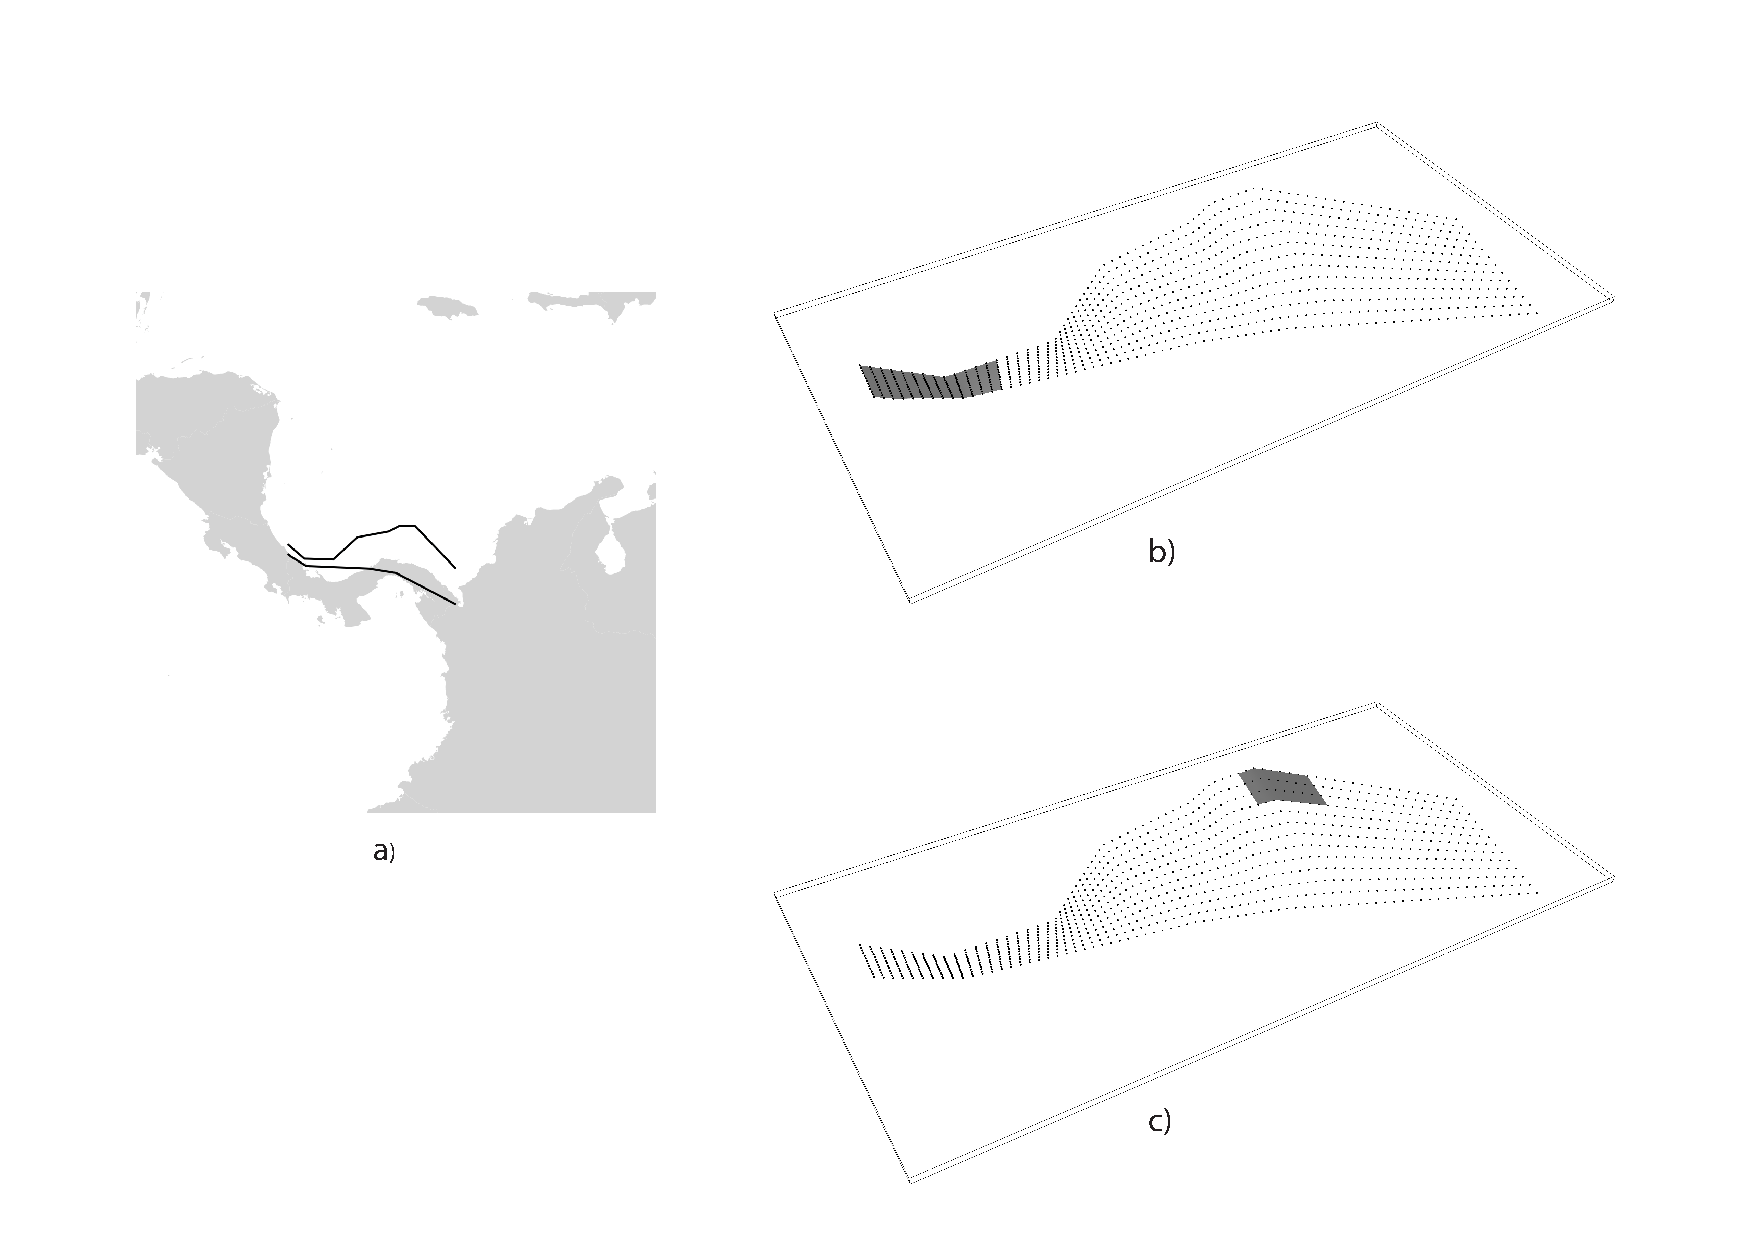
\includegraphics[width=14cm]{./Pictures/ComplexFaultPanama.pdf}
\caption{a) Example of Complex Fault source representing subduction interface fault in North of Panama (PETERSEN2010). The mesh modeling a $M=7.7$ event is depicted in the eastern part b) and in the western part c)}
\label{fig:ComplexFaultSourcePanama}
\end{figure}

\section{The Characteristic Fault source}
The \textit{Characteristic Fault} source is meant to represent individual faults or fault segments that tend to
produce essentialy same size earthquakes (SCHWARTZ COPPERSMITH 1984). To offer the greatest flexibility
in the definition of the associated geometry, a Characteristic Fault can be defined in terms of a simple fault
geometry or as a complex fault geometry. A third option is available, that is a collection of planar ruptures,
which can be used to model multi-segment ruptures for instance (Figure \ref{fig:CharacteristicFaultSource}). In a Characteristic fault, earthquake ruptures
always break the entire fault surface, therefore the rupture floating mechanism is not needed.
\begin{figure}
\centering
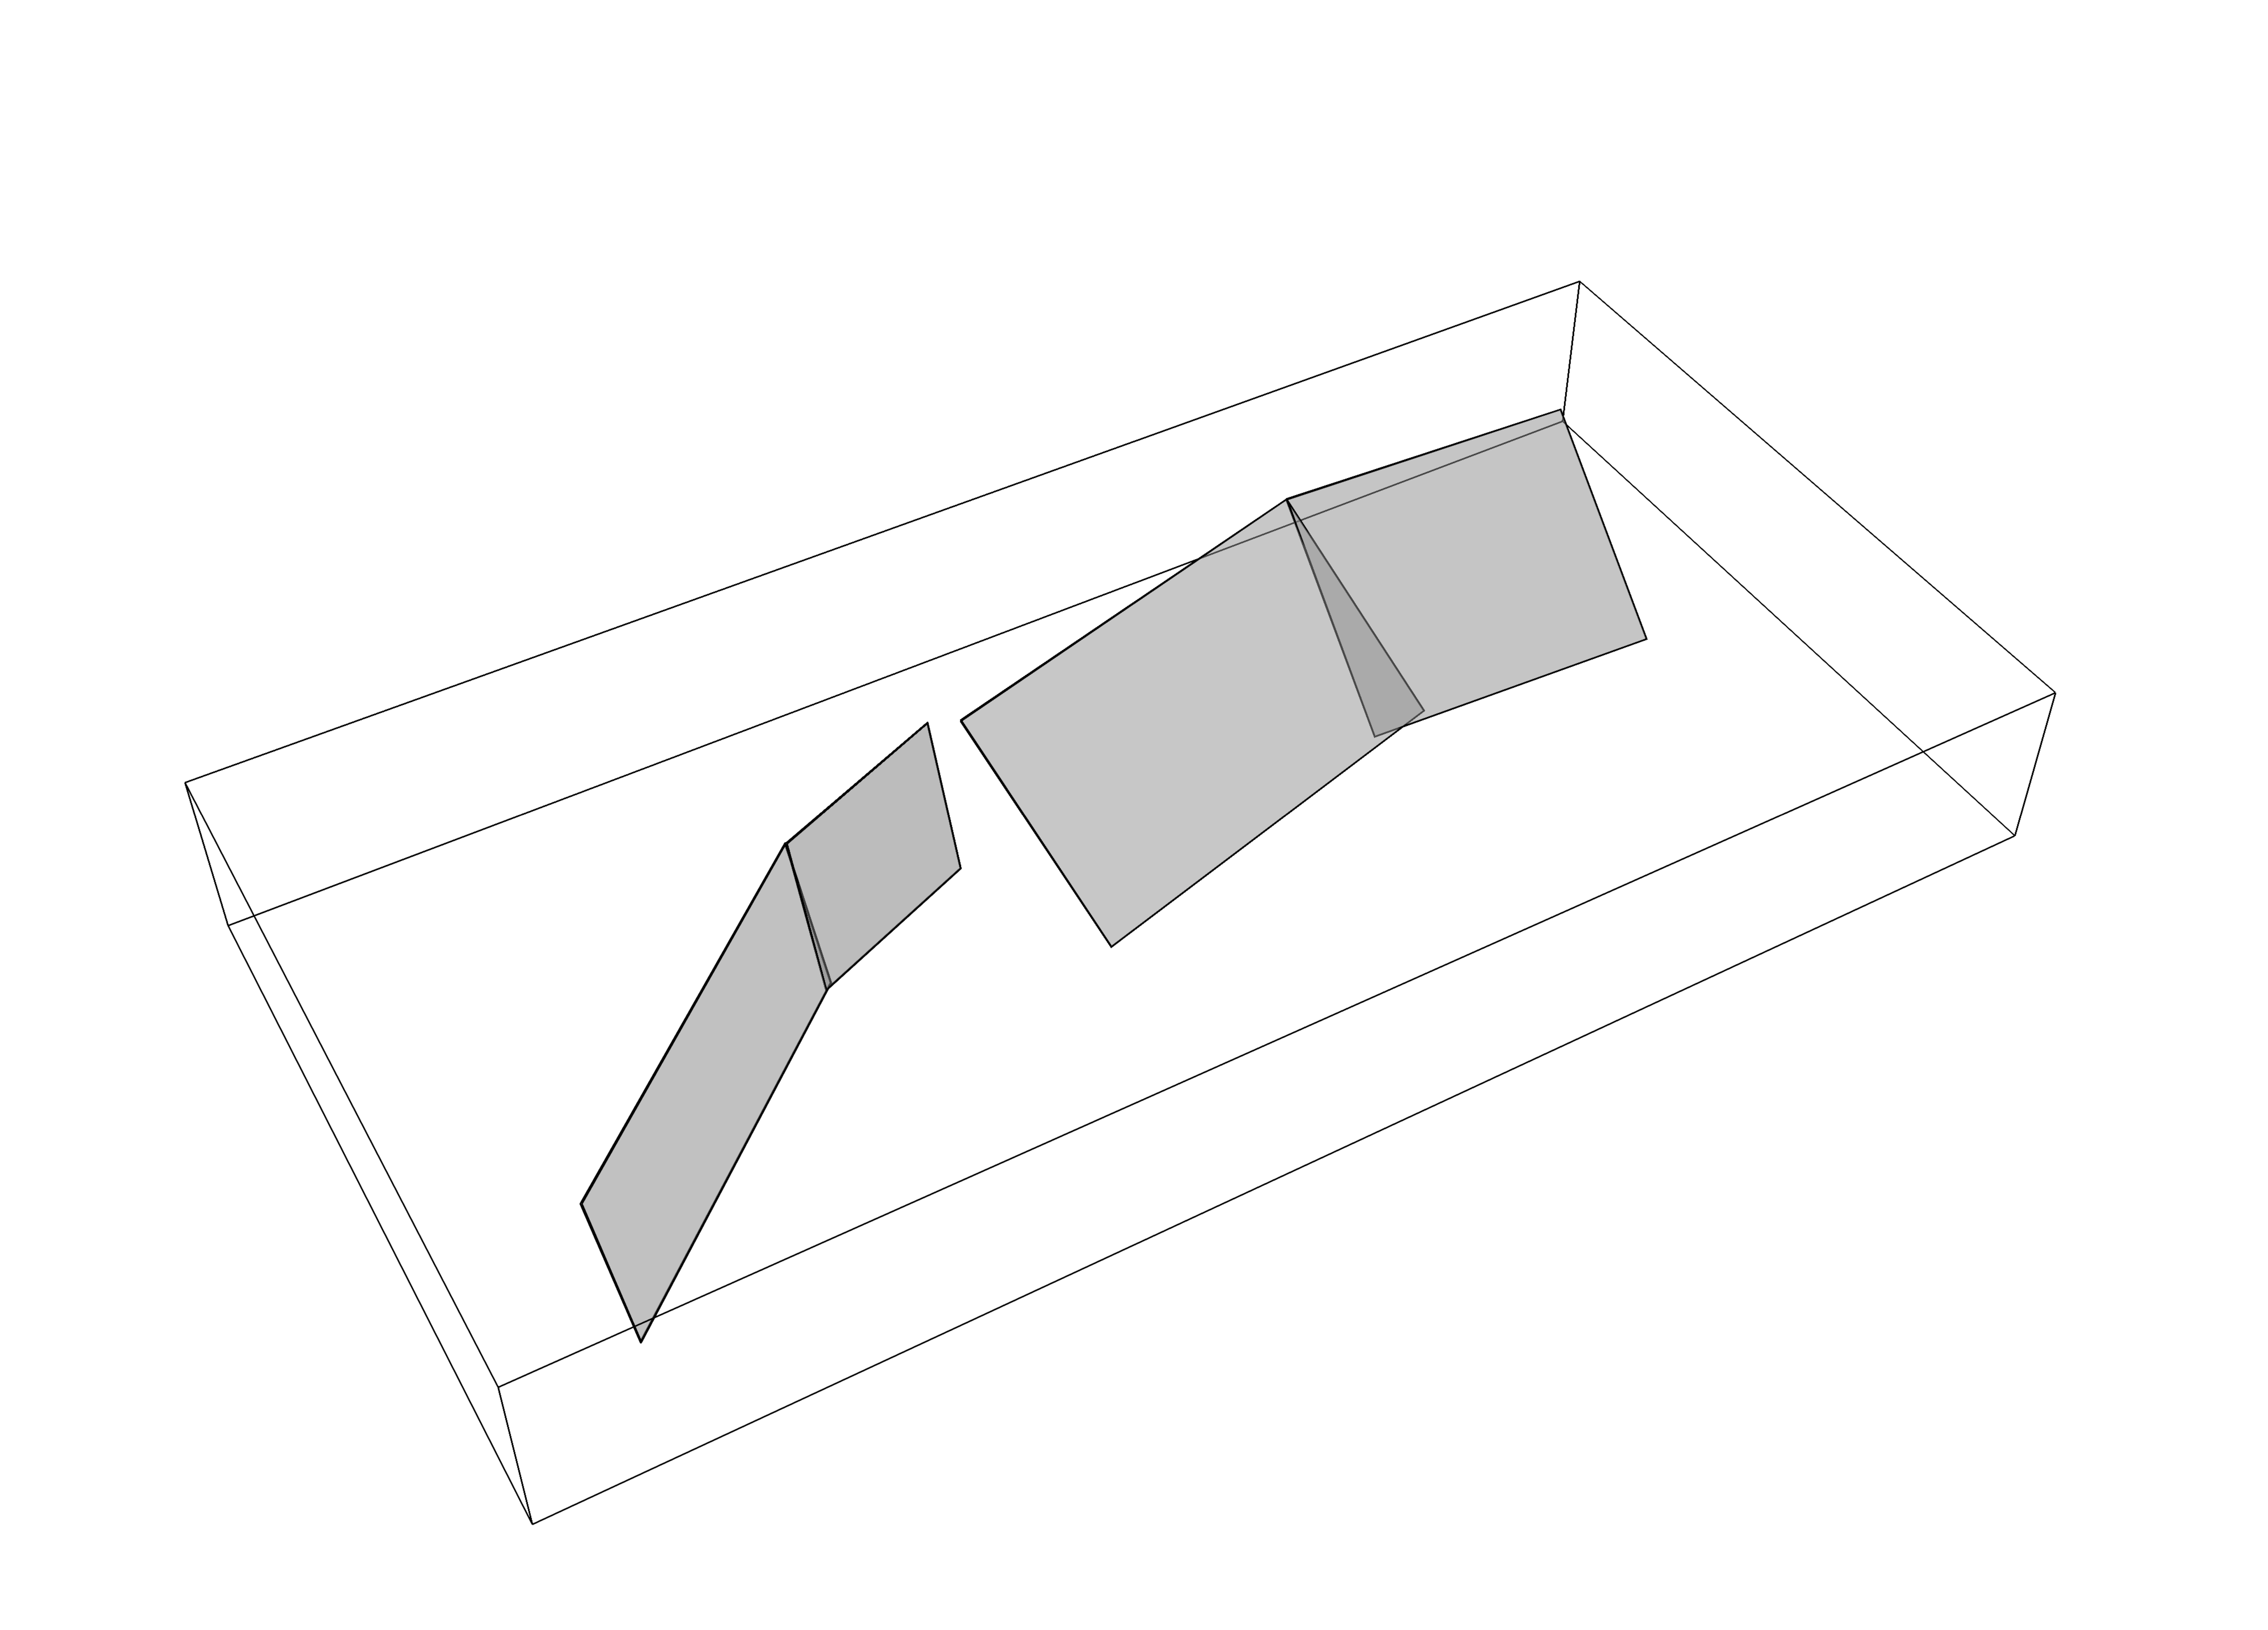
\includegraphics[width=14cm]{./Pictures/CharacteristicFaultSource.pdf}
\caption{Example of Characteristic Fault sources defined through a collection of planar surfaces modeling a multi-segment rupture}
\label{fig:CharacteristicFaultSource}
\end{figure}
%
% ..............................................................................
%\section{Temporal occurrence model}
%\subsection{The Poisson model}
%\index{Temporal occurrence models!Poisson}
%
% ..............................................................................
%\section{Seismic sources for distributed seismicity modelling}
%\index{Distributed seismicity}
%
%Distributed seismicity is the seismicity can cannot be associated unambiguously
%to a specific fault structure.

%\subsection{The point source}
%\index{Seismic source!Point}
%
%\subsection{Area source}
%\index{Seismic source!Area}
%
% ..............................................................................
%\section{Fault sources}
%
%\subsection{Simple fault}
%\index{Seismic source!Simple fault}
%
%\subsection{Complex fault}
%\index{Seismic source!Complex fault}
%
%\subsection{Characteristic fault}
%\index{Seismic source!Characteristic fault}
%
%\section{Non-parametric sources}
%\index{Seismic source!Non-parametric}
